\begin{figure}[p]\centering
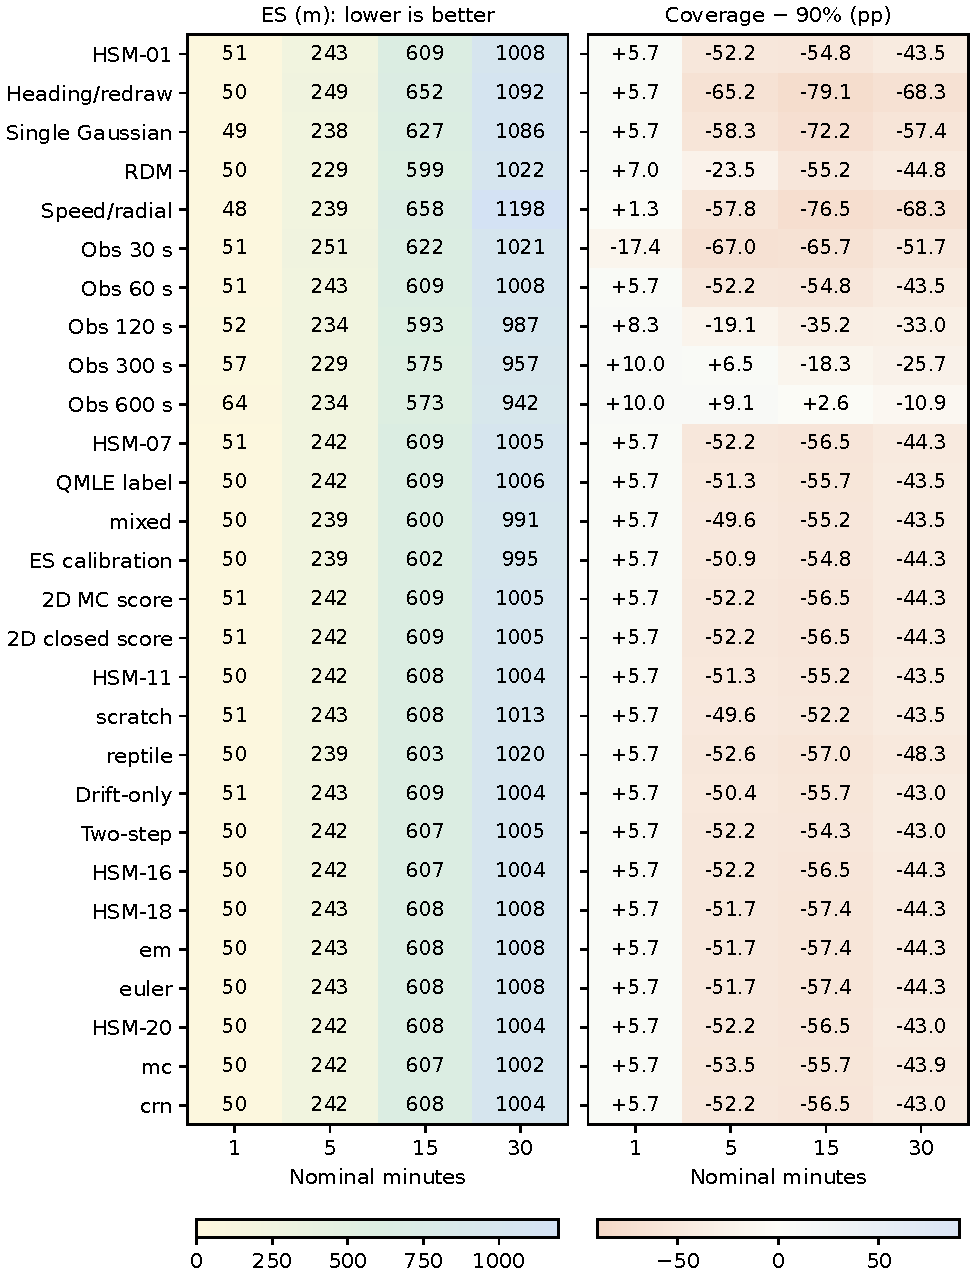
\includegraphics[height=.79\textheight,width=\linewidth,keepaspectratio]{../figures/reader-v9/method-horizon-overview.pdf}
\caption{28 configurations by four horizons by two metrics: 224 scalar cells.
Left: ES (m), lower is better. Right: observed coverage minus nominal 90\%
(percentage points), where zero is the reference and equal positive/negative
departures use equal colour distance. Each cell averages five seeds within
each of 46 blocks, then blocks equally. Original configuration ordering and
separate HSM roles are retained; no performance ranking or new test.
Black numbers and pale linear scales match the main overview. HSM coverage
percentages and precision remain in Table~\ref{tab:all-method-horizons}.}
\label{fig:all-method-horizons}\end{figure}
